\documentclass[10pt]{beamer}
\usetheme[
%%% option passed to the outer theme
%    progressstyle=fixedCircCnt,   % fixedCircCnt, movingCircCnt (moving is deault)
  ]{Feather}
  
% If you want to change the colors of the various elements in the theme, edit and uncomment the following lines

% Change the bar colors:
%\setbeamercolor{Feather}{fg=red!20,bg=red}

% Change the color of the structural elements:
%\setbeamercolor{structure}{fg=red}

% Change the frame title text color:
%\setbeamercolor{frametitle}{fg=blue}

% Change the normal text color background:
%\setbeamercolor{normal text}{fg=black,bg=gray!10}

%-------------------------------------------------------
% INCLUDE PACKAGES
%-------------------------------------------------------

\usepackage[utf8]{inputenc}
\usepackage[english]{babel}
\usepackage[T1]{fontenc}
\usepackage{helvet}

%-------------------------------------------------------
% DEFFINING AND REDEFINING COMMANDS
%-------------------------------------------------------

% colored hyperlinks
\newcommand{\chref}[2]{
  \href{#1}{{\usebeamercolor[bg]{Feather}#2}}
}

%-------------------------------------------------------
% INFORMATION IN THE TITLE PAGE
%-------------------------------------------------------

\title[] % [] is optional - is placed on the bottom of the sidebar on every slide
{ % is placed on the title page
  \textbf{New memory management}
}

\subtitle[SpaceJMP a new approach]
{
}

\author[Rodrigo Siqueira Jordão]
{      Rodrigo Siqueira Jordão \\
      {\ttfamily siqueira@kuniri.org}
}

\institute[]
{
  University of Sao Paulo\\
  Institute of Mathematics and Statistics\\
  
  %there must be an empty line above this line - otherwise some unwanted space
  % is added between the university and the country (I do not know why;( )
}

\date{\today}

%-------------------------------------------------------
% THE BODY OF THE PRESENTATION
%-------------------------------------------------------
\begin{document}

%-------------------------------------------------------
% THE TITLEPAGE
%-------------------------------------------------------

{\1% % this is the name of the PDF file for the background
% the plain option removes the header from the title page, noframenumbering removes the numbering of this frame only
\begin{frame}[plain,noframenumbering] 
  \titlepage % call the title page information from above
\end{frame}}

\begin{frame}[shrink]{Content}{}
  \tableofcontents
\end{frame}

%=======================================================
\section{Context}
%=======================================================
\begin{frame}{Context}{Process-centric}
  % TODO: Create a good image -> Idea: Some thing similar to solar system view
  \begin{figure}[ht]
    \centering
    
\includegraphics[width=0.5\textwidth, keepaspectratio=true]{images/processor-centric.png}
  \end{figure}
\end{frame}

\begin{frame}{Context}{Process-centric}
  \begin{figure}[ht]
    \centering
    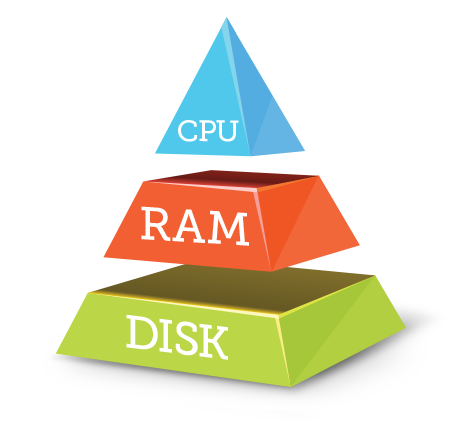
\includegraphics[width=0.5\textwidth, keepaspectratio=true]{images/memory_hierarchy.png}
  \end{figure}
\end{frame}

\begin{frame}{Context}{Memory hierarchy}
  \begin{figure}[ht]
    \centering
    
\includegraphics[width=0.5\textwidth, keepaspectratio=true]{images/memory_hierarchy_why.png}
  \end{figure}
\end{frame}

%=======================================================
\section{Virtual Memory}
%=======================================================
\begin{frame}{Virtual Memory}{Overview}
  % TODO: Create a good image -> Idea: Create your own code
  \begin{figure}[ht]
    \centering
    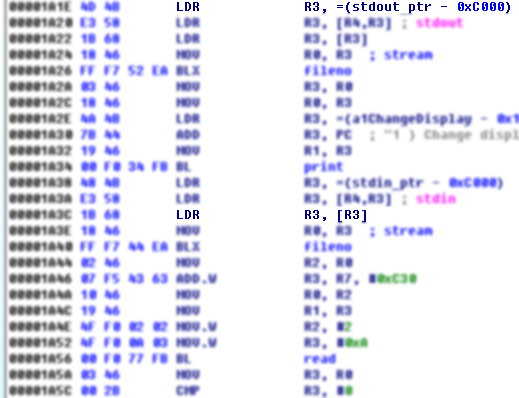
\includegraphics[width=0.5\textwidth, keepaspectratio=true]{images/assembly_code_load_from_memory.png}
  \end{figure}
\end{frame}

\begin{frame}{virtual memory}{overview}
  % TODO: create a good image -> idea: break it in steps to your explanation
  \begin{figure}[ht]
    \centering
    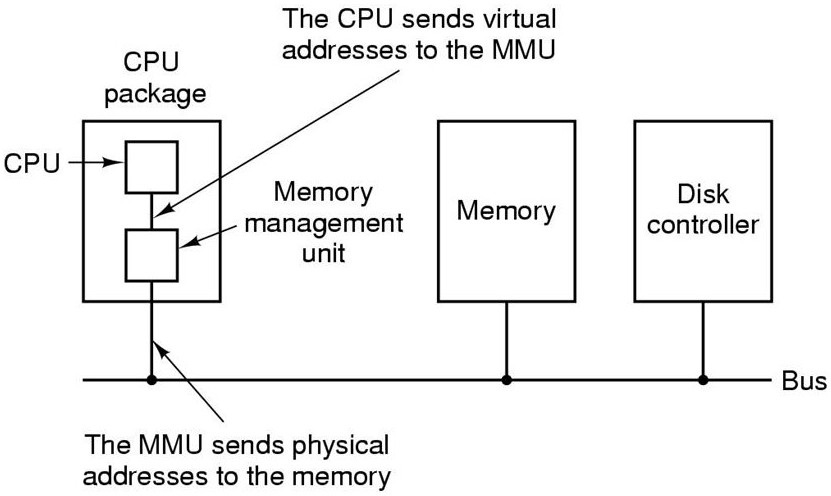
\includegraphics[width=0.5\textwidth, keepaspectratio=true]{images/mmu_cpu.png}
  \end{figure}
\end{frame}

\begin{frame}{virtual memory}{overview}
  % TODO: create a good image -> idea: break it in steps to your explanation
  \begin{figure}[ht]
    \centering
    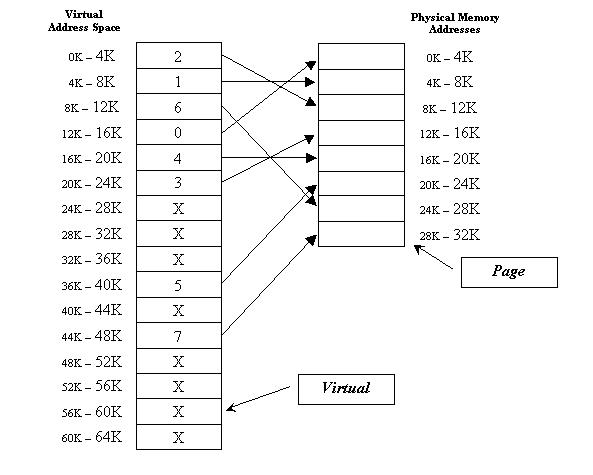
\includegraphics[width=0.5\textwidth, keepaspectratio=true]{images/virtual_memory.png}
  \end{figure}
\end{frame}

{\1
\begin{frame}[plain,noframenumbering]
  \finalpage{Thank you!}
\end{frame}}

\end{document}
